%% ============================================================================
%% ============================================================================
\begin{frame}[plain]{Subproduct trees}
\fontsize{8}{9}\selectfont  
{
\begin{itemize}
	\item Useful construction to devise \textcolor{blue}{fast algorithms} with univariate polynomials,
	\item If $m_0, m_1,\ldots , m_{n-1}$ are monic, non-constant, polynomials in ${\K}[x]$, then their subproduct tree can be constructed in $O(M(d)\log_2(n))$ operations in {\K}
where  $d = \sum_{i=0}^{n-1}\degree{m_i}$.
\end{itemize}
}	
\begin{figure}[htb] %htb
  \begin{center}
  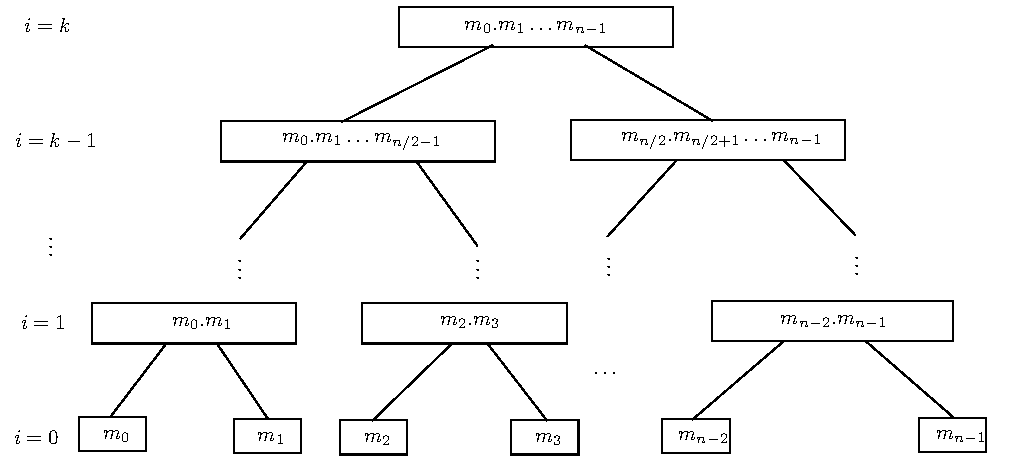
\includegraphics[scale=0.6]{images/sptree2.pdf} %width=6.4in,height=3.0in
  \end{center}
\end{figure}	
\end{frame} 
%% ============================================================================
%% ============================================================================
\begin{frame}[plain]{Fast multiple remainders}

\fontsize{8}{9}\selectfont  
{
\begin{itemize}
\item Let $m_0, m_2,\ldots , m_{n-1}$ be as before and assume their subproduct tree $M$
      has been computed. Let $f \in {\K}[x]$ be a polynomial of degree less than $d$.
\item To compute $f  \ {\rm rem} \ m_0, f  \ {\rm rem} \ m_1,\ldots , f  \ {\rm rem} \ m_{n-1}$, 
      one reduces $f$ by the root of $M$, then by its children (leading to two remainders)
      and so on.
\item This amounts to $O(M(d)\log_2(n))$ operations in {\K}.
\end{itemize}
}

\begin{figure}[htb] %htb
  \begin{center}
  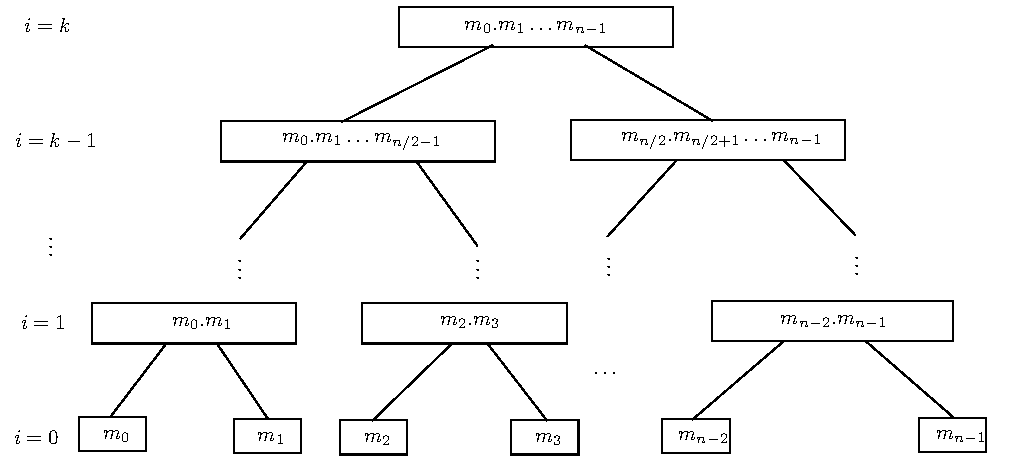
\includegraphics[scale=0.5]{images/sptree2.pdf} %width=6.4in,height=3.0in
  \end{center}
\end{figure}

\end{frame} 
%% ============================================================================
%% ============================================================================
\begin{frame}[plain]{Fast evaluation}

\fontsize{8}{9}\selectfont  
{
\begin{itemize}
\item Suppose the polynomials $m_0, m_2,\ldots , m_{n-1}$ are of the form
      $x - x_0, x- x_1, \ldots, x - x_{n-1}$, where
      $x_0, x_1, \ldots, x_{n-1}$ are pairwise values in {\K}.
\item In this case, the procedure for fast multiple remainders
      provides a procedure for \blue{mulit-point evaluation}
      running in $O(M(d)\log_2(d))$ operations in {\K}.
\item This is a significant improvement w.r.t Horner's Rule
      which runs in $O(d^2)$ operations in {\K}.
\end{itemize}
}

\begin{figure}[htb] %htb
  \begin{center}
  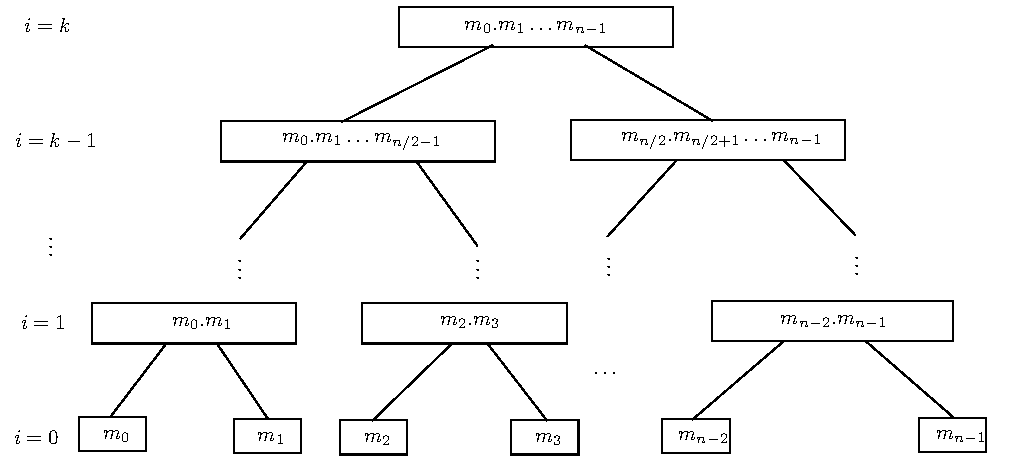
\includegraphics[scale=0.5]{images/sptree2.pdf} %width=6.4in,height=3.0in
  \end{center}
\end{figure}

\end{frame} 
